%-%-%-%-%-%-%-%-%-%-%-%-%-%-%-%-%-%-%-%-%-%-%-%-%-%
% EE531: laboratório de Eletrônica Básica I       %  
% Experimento 1: Familizarização com instrumentos %
%                de medida                        %
% Data:07/08/2010                                 %
% Unicamp,Campinas,São Paulo,Brasil               % 
% Grupo:                                          %
%       - Raquel Mayumi Kawamoto                  %
%       - Tiago Chedraoui Silva                   % 
%-%-%-%-%-%-%-%-%-%-%-%-%-%-%-%-%-%-%-%-%-%-%-%-%-%
%\documentclass[letter]{article}  % formato impressao IC
\documentclass[a4paper]{article} % formato impressao FEEC

%%% fontes %%%
\usepackage[T1]{fontenc}
\usepackage[brazil]{babel}    % dá suporte para os termos na língua portuguesa do Brasi
\usepackage[utf8]{inputenc}   % acentuação
\usepackage{ae,aecompl,aeguill}       % pdfs mais bonitos =)

%%% outros %%%
\usepackage{multirow}
\usepackage{textcomp}
\usepackage{color}       
\usepackage{indentfirst}      % retira padrao americano de paragrafos
\usepackage{multicol}   
\usepackage[linkbordercolor={1 1 1},urlcolor=black,colorlinks=true]{hyperref} % links

% circuito eletrico
\usepackage{electComp}
\usetikzlibrary{decorations,decorations.pathmorphing,decorations.pathreplacing}
\usepackage{verbatim}
\usepackage{pstricks}

\usepackage[letterpaper]{geometry}
\geometry{verbose,lmargin=3cm,rmargin=3cm}

\date{Agosto 20, 2010}
% Capa estilizada %
\newcommand*{\titleTMB}{\begingroup \centering \settowidth{\unitlength}{\LARGE EE531} {\large\scshape EE531 - Turma S}\\[0.2\baselineskip] \rule{11.0cm}{1.6pt}\vspace*{-\baselineskip}\vspace*{2pt} \rule{11.0cm}{0.4pt}\\[\baselineskip] {\LARGE  Familizarização com instrumentos de medida}\\\vspace*{\baselineskip}  {\itshape Laboratório de Eletrônica Básica I - Segundo Semestre de 2010}\\ \rule{11.0cm}{0.4pt}\vspace*{-\baselineskip}\vspace{3.2pt} \rule{11.0cm}{1.6pt}\\[\baselineskip] {\large\scshape Professor: José Cândido Silveira Santos Filho}\par \vfill {\normalsize   \scshape 
    \begin{center} 
      \begin{tabular}{  l  l  p{5cm} } 
        Raquel Mayumi Kawamoto & RA: 086003\\
        Tiago Chedraoui Silva  & RA: 082941\\
      \end{tabular} \end{center}
    \itshape \today   }\\[\baselineskip] \vspace{3.2pt} \endgroup}


\begin{document}
\titleTMB 
\newpage
%Amplitude pico-à-pico 9.8 V
%período 100 micros
%tempo de subida
%tempo de descida 40 micro segundos 
%offset +1 v+ +2
%          v- +2
%offset -1 v+ -2
%          v- -2

%Vrms 2.88 V
%Vavg -57.1 mV
%Vpp 9.92V
%Prd 100 micro
%Rise 42 micro seg
%Fall 42 micro seg


Para este experimento inicial da disciplina de laboratório de eletrônica básica I, tem-se como objetivo a familiarização dos alunos com os diversos instrumentos que serão utilizados ao longo do curso. Estas ferramentas são a fonte de alimentação dual, um gerador de funções e um osciloscópio digital. Para este presente experimento utilizam-se ainda um protoboard, dois resistores de 
$100k\Omega$ e dois capacitores de $100pF$. 
	

\section*{Parte Experimental}
\begin{enumerate}
\item Para esta parte inicial do experimento, a saída do gerador de funções é conectada ao canal 1 do osciloscópio. O gerador é ajustado para produzir um sinal de tensão com sua forma de onda triangular, com amplitude 10$V_{pp}$, com offset de $0V$ e frequência de $10kHz$. 
 
Com o recurso \textit{cursor} do osciloscópio, foi medida a amplitude de pico-a-pico, o período, o tempo de subida e o tempo de descida do sinal de tensão. Tais dados encontram-se na tabela \ref{tab:cursors}. 


%\begin{figure}[h]
%\begin{centering}
%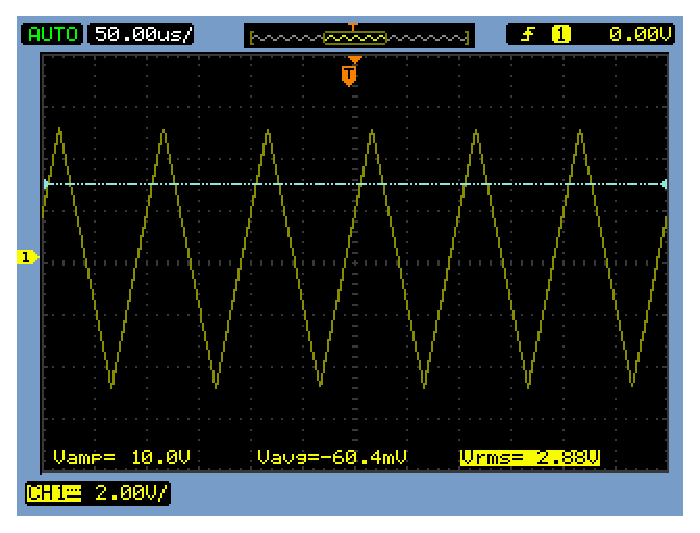
\includegraphics{Imagens/412}\caption{Figura 412 \label{fig:Fig-412}}
%\par\end{centering}
%\end{figure}

\begin{figure}[h]
\begin{centering}
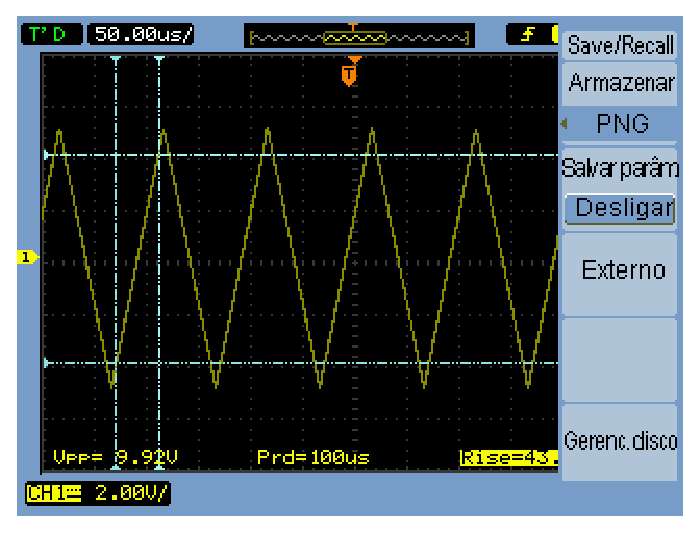
\includegraphics[scale=0.8]{Imagens/4122}\caption{Medição do tempo de subida \label{fig:Fig-4122}}
\par\end{centering}
\end{figure}

\begin{table}[h]
\begin{centering}
\caption{Dados experimentais obtidos através do recurso \textit{cursor} \label{tab:cursors}}

\begin{tabular}{cc}
\hline 
Descrição & Valor\tabularnewline
\hline
Amplitude pico-a-pico & 9,8V\tabularnewline
Período & 100$\mu s$\tabularnewline
Tempo de subida & 40$\mu s$\tabularnewline
Tempo de descida  & 40$\mu s$\tabularnewline
\hline
\end{tabular}
\par\end{centering}

\end{table}

%Ao configurar o canal para medida a.c., no qual o sinal é filtrado de forma a obter somente a componente variável do sinal, e, posteriomente, configurar para medida c.c, não se constatou grandes diferenças entre os valores.
Para comparar as componentes contínuas e variáveis de um sinal, é possível configurar o canal tanto para medidas a.c, no qual o sinal é filtrado de forma a obter somente a componente variável do sinal, quanto para c.c, no qual o sinal contém tanto a componente variável quanto contínua. Utilizando ambas configurações, não se constatou grandes diferenças entre os sinais, ou seja, componente contínua do sinal é pequena. \\
Além disso, ao alterar a tensão de offset para 1 volts, a componente contínua do sinal de entrada aumentou 2 volts, e ao alterar para -1 volts, a componente contínua do sinal de entrada diminui 2 volts. 

Em seguida, os mesmos valores da tabela \ref{tab:cursors} foram medidos, porém usando-se o recurso measure (figura \ref{fig:Fig-1}), além de também ser necessário medir o valor médio e o valor RMS (ambos os valores obtidos também com o recurso measure). Tais dados encontram-se na tabela \ref{tab:measure} .\\ 

\begin{figure}[h!]
\begin{centering}
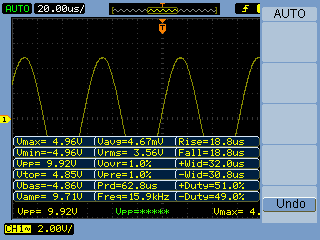
\includegraphics[scale=0.7]{Imagens/1}\caption{Caracterização da onda através do recurso measure \label{fig:Fig-1}}
\par\end{centering}
\end{figure}

\begin{table}[h]
\begin{centering}
\caption{Dados experimentais obtidos através do recurso measure \label{tab:measure}}
\begin{tabular}{cc}
\hline 
Descrição & Valor\tabularnewline
\hline
Amplitude pico-a-pico & 9,92V \tabularnewline
Período & 100$\mu s$\tabularnewline
Tempo de subida & 42$\mu s$\tabularnewline
Tempo de descida  & 42$\mu s$\tabularnewline
$V_{avg}$ & -57,1 mV\tabularnewline
$V_{rms}$ & 2,88V \tabularnewline
\hline
\end{tabular}
\par\end{centering}
\end{table}
\newpage
Os valores obtidos através do recurso cursor com os dos obtidos com o do recurso measure são valores bem semelhantes e próximo um do outro, com a diferença de que os dados adquiridos com o cursor são menos precisos do que os do medidos com o measure.

\item Para a segunda parte do experimento, calcula-se, através da equação 1,
\vspace{1mm}

\begin{equation}
 f_{c}=\frac{1}{2\pi RC}\\
\end{equation}

\vspace{2mm}


 a frequência de corte para cada filtro do circuito esquemático da figura \ref{tab:circ}, na qual o circuito à esquerda da fonte de sinal é um filtro passa-altas com constante de tempo simples (CTS), e à direita da fonte é um circuito passa-baixas, também CTS. Assim, obtém-se para os circuitos uma frequência de corte equivalente a 15,92 KHz.


\vspace{3mm}
\begin{figure}[h]
\centerline{\input circ.tex}
\caption{Circuito \label{tab:circ}}
\end{figure}

\vspace{2mm}


\item Para a parte três, foi montado, no protoboard, o circuito da figura do item anterior. Inicialmente, a onda triangular foi substituída por uma onda senoidal de amplitude $10V_{pp}$, offset de $0V$ e frequência de $16kHz$. Este sinal foi aplicado ao nó 1 do circuito. Sendo assim, efetuou-se as medidas necessárias, completando a tabela \ref{tab:Medidas-do-filtro} (tabela de medidas de filtro CTS).

\begin{figure}[h]
\begin{centering}
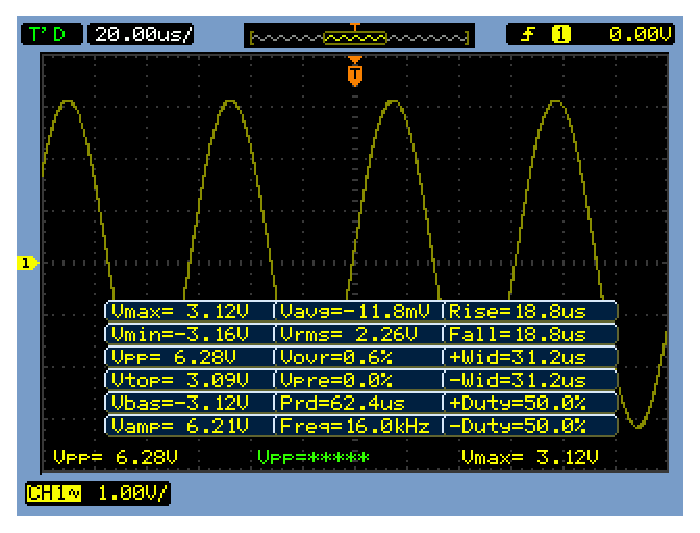
\includegraphics[scale=0.7]{Imagens/3}\caption{Sinal no nó 3 \label{fig:Fig-3}}
\par\end{centering}
\end{figure}

%
\begin{table}[h]
\begin{centering}
\caption{Medidas do filtro CTS \label{tab:Medidas-do-filtro}}
\begin{tabular}{|c|c|c|c|}
\hline 
Nó & 1 & 2 & 3\tabularnewline
\hline
\hline 
Amplitude pico-a-pico & 9,92V  & 6,28V  & 6,48V \tabularnewline
\hline 
Valor médio & 2,40mV & -13,5mV  & -12,7mV \tabularnewline
\hline 
Valor RMS & 3,56V & 2,26V  & 2,32V \tabularnewline
\hline 
Valor máximo & 4,96V & 3,12V  & 3,24V \tabularnewline
\hline 
Valor mínimo & -4,96V  & -3,16V  & -3.24V \tabularnewline
\hline
\end{tabular}
\par\end{centering}


\end{table}

\item                Em seguida, aplicando-se um sinal senoidal de amplitude  $10V_{pp}$, um offset de 0V e variando-se a frequência segundo a tabela \ref{tab:var-freq}, obtiveram-se os dados contidos na mesma tabela (tabela 4). Em baixas frequências,  a fase no nó 2 aumenta sendo o seu máximo, para os casos considerados, de 90$^{\circ}$. Já o nó 3 apresenta uma diminuição na fase. Para a mínima frequencia considerada, sua fase é de 0$^{\circ}$.  Aumentando-se a frequência, a fase do nó 2 relativa ao nó 1 diminui e, para a máxima frequencia, ela atinge uma fase mínima de 0$^{\circ}$. Diferentemente a este nó, a fase relativa do nó 3 em relação ao nó 1 aumenta – em módulo – atingindo 90$^{\circ}$ para  a frequencia de 1MHz.
                Com relação a variação na frequência de entrada $V_{in}$, quando há um aumento em sua frequência, a amplitude (pico a pico) do nó 2 aumenta,  enquanto que a do nó 3 diminui.  




%Em seguida, foi aplicado um sinal senoidal de amplitude $10V_{pp}$, com offset de 0V e variou-se a frequência conforme a tabela \ref{tab:var-freq}. 
%Ao diminuir a frequência de entrada $V_{in}$, a amplitude do sinal no nó 3 aumenta enquanto no nó 2 diminui. Além disso, a fase no nó 2 aumenta, alcançando, em baixas frequências, uma fase de 90$^{\circ}$,enquanto no nó 3 a fase diminui alcançando, em baixas freqüências, uma fase de  0$^{\circ}$.
%Por outro lado, ao aumentar a frequência de entrada $V_{in}$, a amplitude do sinal no nó 3 aumenta, enquanto no nó 2 diminui, e a fase no nó 2 diminui, alcançando em altas frequências uma fase de 0$^{\circ}$, já no nó 3, a fase diminui, alcançando, em altas frequências, uma fase de 90$^{\circ}$.   

%
\begin{table}[h]
\begin{centering}
\caption{Medidas realizadas variando-se a frequência do sinal \label{tab:var-freq}}
\begin{tabular}{|c|c|c|c|c|c|c|c|}
\hline 
Nó & frequência & 100 Hz & 1kHz & 10kHz & 16kHz & 100kHz & 1MHz\tabularnewline
\hline
\hline 
1 & Amplitude pico-a-pico & 10,2V & 10,2V  & 10,2V & 10,2V & 10,2V  &10,2V \tabularnewline
\hline 
\multirow{3}{*}{2}
 & Amplitude pico-a-pico & 100mV & 656mV & 4,8V & 6,24V & 8,40V & 8,48V \tabularnewline
\cline{2-8} 
 & \multicolumn{1}{c|}{Ganho em dB} & -40,17 & -23,83  & -6,55 & -4,27  & -1,69  & -1,60 \tabularnewline
\cline{2-8} 

 & Fase relativa ao nó 1 & $90^{\circ}$ & $86^{\circ}$  & $56^{\circ}$  & $41^{\circ}$  & $7^{\circ}$  & $0^{\circ}$ \tabularnewline
\hline 
\multirow{3}{*}{3}
 & Amplitude pico-a-pico & 10,4v & 9,8V & 7,76V & 6,32V  & 1,42V  & 180mV \tabularnewline
\cline{2-8} 
 
 & Ganho em dB &  0,17 & -0,35  & -2,37 & -4,16 & -17,13 & -35,07\tabularnewline
\cline{2-8} 
 
 & Fase relativa ao nó 1 & $0^{\circ}$ & $-3^{\circ}$ & $-36^{\circ}$  & $-46^{\circ}$  & $-72^{\circ}$  & $-90^{\circ}$ \tabularnewline
\hline
\end{tabular}
\par\end{centering}

\end{table}

\item Ao comparar um circuito passa-baixa e um passa-alta determina-se que as diferenças de fases, independentemente da frequência, vale 90 $-3^{\circ}$.
Portanto, quando o valor do sinal em um circuito estiver em seu máximo, no outro estará no zero. Assim, ao realizar uma diferença de nas medidas da tensão diferencial entre o nó 2 e o nó 3, devemos obter uma senóide cujo pico valha a soma do maior dos picos entre as ondas no nós 2 e 3. Como o valor pico-a-pico do nó 2 vale 4,80V e no nó 3 7,76V, o valor pico a pico da onda resultante da diferença entre elas possuiria valor de 7,76V.
Contudo, conforme a figura \ref{fig:Fig-45}, a diferença de fase obtida é um pouco maior que $90^{\circ}$. Logo o valor pico a pico ficou um pouco acima do esperado, atingido em módulo 9,12V, o que pode ser explicado já que ao aumentar a diferença entre as fases, quando um está no máximo o outro está  abaixo do eixo das abscissas, o que incrementa o valor da senóide resultante.        

\begin{figure}[h]
\begin{centering}
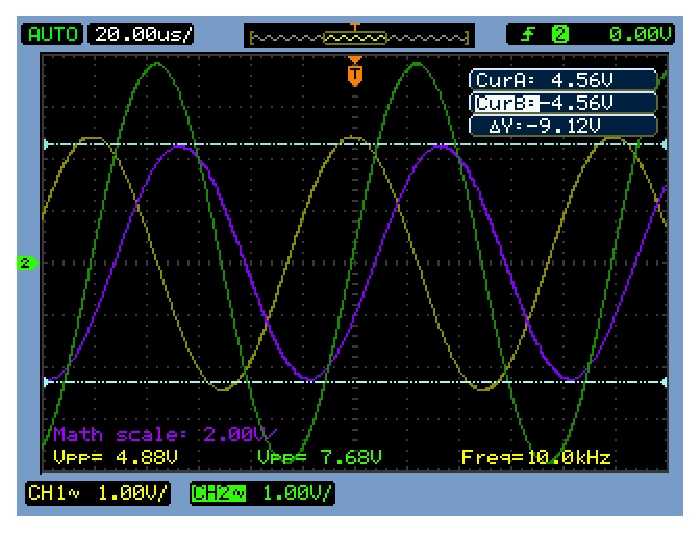
\includegraphics[scale=0.7]{Imagens/45} \caption{Medida da tensão diferencial entre os nós 2 e 3 \label{fig:Fig-45}}
\par\end{centering}
\end{figure}

\end{enumerate}

\end{document}
